We now consider a subset of cluster management closely related to
this thesis' goal of ensuring efficient resource utilization and quality of
service. Specifically, we introduce
auto-scaling, a method of ensuring each application has the necessary amount
of computational resources to handle varying external
demands.

To better understand both the implementation and benefits of auto-scaling, let
us consider a simple scenario. Imagine you have an application running on a
cluster for a week. On Monday, it will need $x$ resources.\footnote{By
  \textit{resources}, we mean CPU, memory, etc.} On Tuesday through
Thursday, the application will need $2x$ resources. Finally, on Friday the
application will again need $x$ resources. Without auto-scaling, we are forced
to assign a constant amount of resources to the application running on our
cluster. However, there is no constant amount of resources that can meet
the two goals of efficiently utilizing the cluster's resources and ensuring the
application has the resources needed for maintaining a high-level of service.
Specifically, if we assign the application $x$ resources,
then on Tuesday through Thursday the
application will not have the amount of resources it needs to handle its load,
and quality of service will deteriorate. Alternatively, if we assign the
application $2x$ resources on the cluster, then on Monday and Friday we will
essentially be wasting $x$ resources on the cluster, as they are assigned to an
application that does not need them. Such waste indicates inefficient
resource utilization. If we desire to run additional jobs on the cluster, we
must allocate more resources, even though our statically over-provisioned
application has plenty of resources it is not using.
The difficulties static resource provisioning suggests can
be seen in Figure \ref{fig:static-over-provision} and Figure
\ref{fig:static-average-provision} \footnote{The graphs showing the
  benefits of auto-scaling are inspired by the informative graphs
showing the benefits of auto-scaling in the Amazon EC2 auto-scaling
documentation.\cite{amazon-ec2}.}

\begin{figure}[!h]
  \centerline{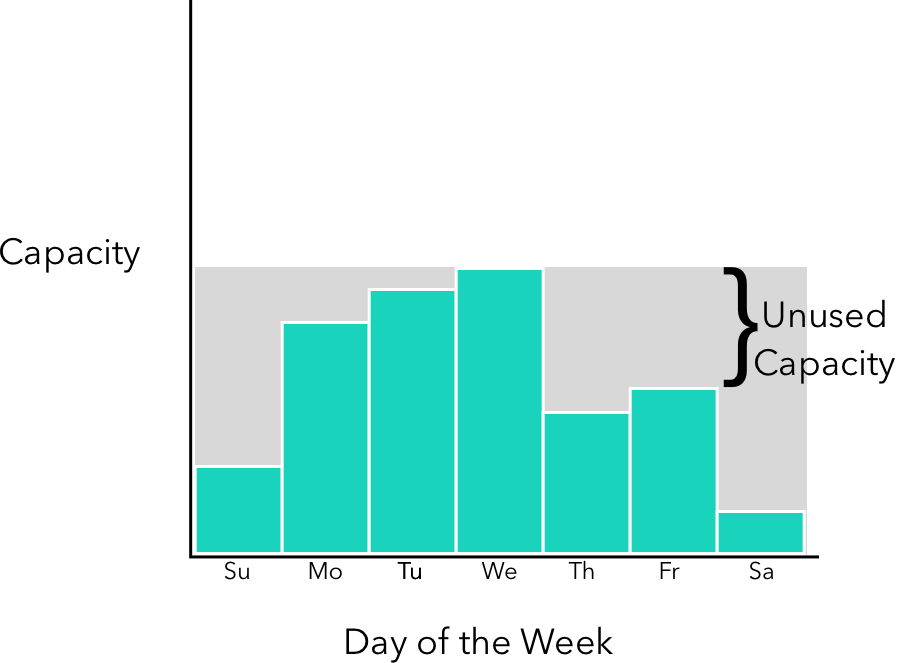
\includegraphics[scale=.25]{static-over-provision.jpg}}
  \caption{A Over Provisioned Application}
  \label{fig:static-over-provision}
\end{figure}

\begin{figure}[!h]
  \centerline{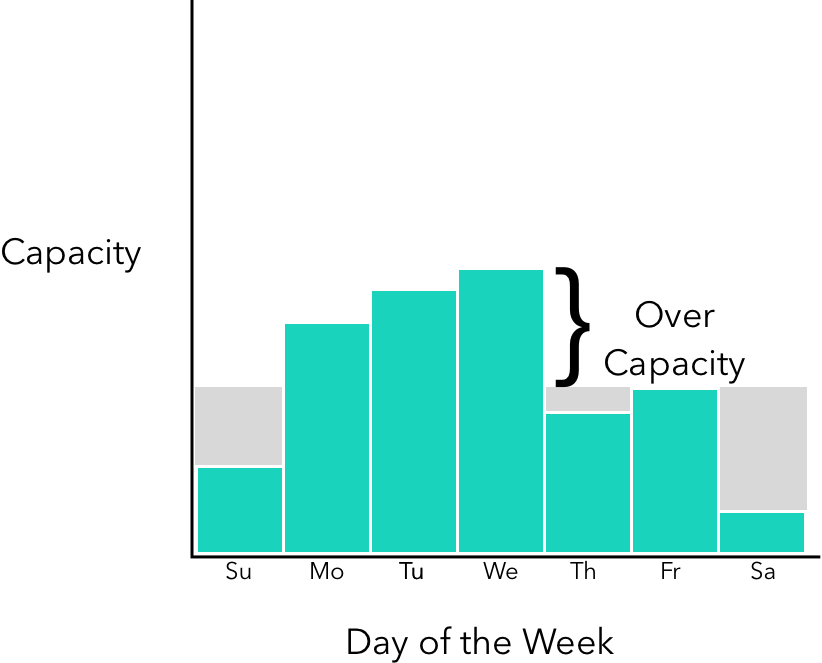
\includegraphics[scale=.25]{static-average-provision.jpg}}
  \caption{A Average Provisioned Application}
  \label{fig:static-average-provision}
\end{figure}

We use auto-scaling to address the inability of statically allocated
resources to efficiently handle all the variances in application load.
Auto-scaling allows us to assign an application more or less resources based on
the status of the cluster. In our previous example, perfect auto-scaling
would allow us to assign the cluster $x$ resources on Monday and Friday and
$2x$ resources on Tuesday through Thursday. Through auto-scaling, we accomplish
both goals: our application has the needed resources for a high quality
of service and our cluster is efficiently utilizing resources by only
allocating the application what it needs. If we desire to run more jobs on our
cluster, they can ``fill-in'' the resources our application relinquishes when it
auto-scales, preventing us from having to purchase more computing power that
will just be wasted at certain times.
Overall, auto-scaling can make applications on a cluster more performant and
the cluster more cost-effective, as can be seen Figure
\ref{fig:reactive-autoscale}.

\begin{figure}[!h]
  \centerline{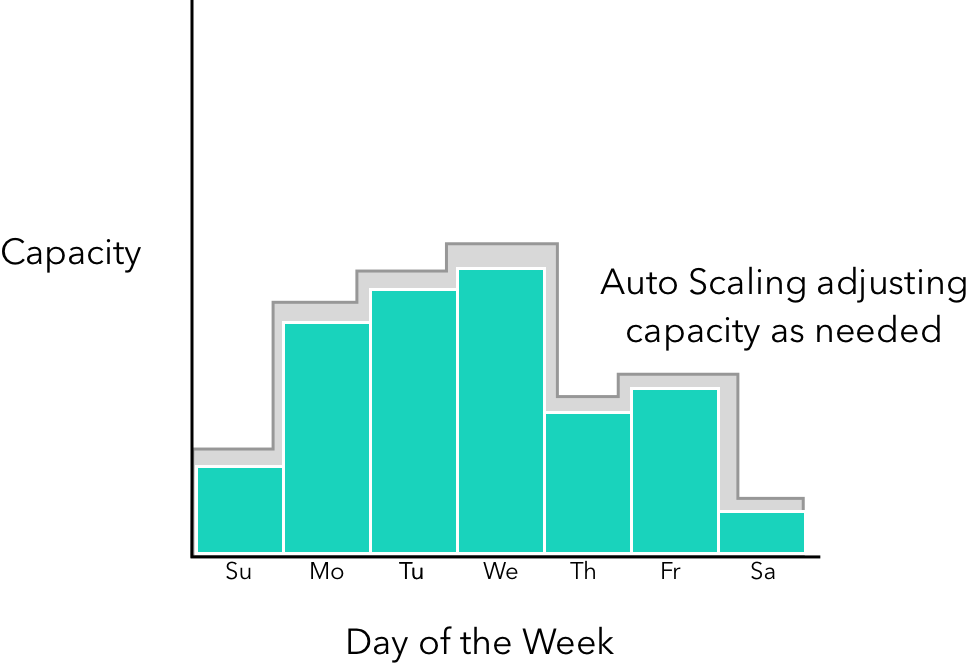
\includegraphics[scale=.25]{reactive-autoscale}}
  \caption{A Reactive Auto-scaled Application}
  \label{fig:reactive-autoscale}
\end{figure}

Given an understanding of the importance of auto-scaling, we now begin to
examine the differing implementations of auto-scaling. Auto-scaling
implementations differ in how the cluster manager
assigns an application the new resources it
needs\footnote{Auto-scaling implementations can also take away resources from
an application running on a cluster.} and how the cluster manager makes its
auto-scaling decisions. Given these two points of
variation, there are two predominant characteristics that shape the nature of an auto-scaling
implementation. The first is if the auto-scaling is horizontal or vertical. The
second is if the auto-scaling is reactive or predictive.

\begin{enumerate}
  \item \underline{Horizontal vs. Vertical}: We begin by examining
    the difference between horizontal and vertical scaling.
    Let us begin by assuming there is an application assigned $x$ resources by the
    cluster manager. The application
    faces external load such that it needs $2x$ resources to operate with an
    acceptable quality of service. There are now two options. In
    \textit{vertical} auto-scaling, the cluster manager will attempt to assign
    the application the needed $2x$ resources
    without halting the execution of the application. In \textit{horizontal}
    auto-scaling, the cluster manager will create another instance of
    the application, so that there are two machines each with
    $x$ resources ($2x$ resources in summation). The load will be split between
    the two new instances of the application, meaning each machine handles half
    the requests and requires only the $x$ resources it has
    \cite{auto-scaling-techniques-for-elastic-applications-in-cloud-environments}. While
    both of these variations of auto-scaling accomplish the same goal, horizontal
    auto-scaling is a little simpler. Given we know how to create an instance of a
    virtual machine running the application, an entirely safe assumption
    considering we already created one such instance, in many cases it is
    fairly trivial to create
    another instance, and then split the load between these two instances using
    standard methods of load balancing.\footnote{Claiming
    simplicity assumes the application is written
    such that it can be replicated with no unexpected modifications
    on operation. For example, a static web server is trivial to horizontally
    auto-scale, while a relational database is not.}
    Historically, vertical auto-scaling has been more complex,
    although that is rapidly changing.
    The complexity of vertical auto-scaling depends on how the application
    is run. If the application is run directly on a fully utilized machine,
    then it is extremely difficult to assign the application more resources
    without stopping it from running, as assigning more resources
    would require transferring a running
    process to a new machine with more abundant resources.\footnote{In reality,
    it would be extremely rare for a cluster manager to run applications
    directly on the nodes of the cluster with no degree of isolation.} The complexity
    slightly decreases, although is still considerable, when the application is
    running on a virtual machine. Virtual machines can claim or relinquish
    resources from their host, thus allowing the application the varying
    resources it needs. KVM, the hypervisor within the Linux kernel, implements
    this process through ``balloon'' drivers \cite{kvm-automatic-ballooning}.
    Finally, if the application is running within a container, performing
    vertical scaling is simple. Linux container implementations allocate
    resources using cgroups, which assign set amounts of resources to certain
    processes. It is possible to modify the cgroup allocation while the process
    is still running, meaning vertical auto-scaling without stopping the
    application is trivial \cite{docker-up-and-running}.
    As containerization becomes increasingly prevalent, the difference in
    difficulty between horizontal and vertical auto-scaling decreases.
    The implementations of auto-scaling we examine focuses on horizontal
    auto-scaling, although the majority of research done for this thesis applies
    to vertical auto-scaling with only minor modifications
    \cite{auto-scaling-techniques-for-elastic-applications-in-cloud-environments}.

  \item \underline{Reactive vs. Predictive}: We continue by
    examining the distinction between reactive and predictive
    auto-scaling. At the simplest level, reactive auto-scaling reacts to
    the current state of the application and cluster, while predictive
    auto-scaling reacts to a prediction of the future state of the application and cluster
    \cite{auto-scaling-techniques-for-elastic-applications-in-cloud-environments}.
    While reactive auto-scaling must only consider one
    time-frame when gathering and interpreting information, predictive
    auto-scaling must consider many different time-frames with respect to the
    most accurate method of projecting past metrics into future metrics. However,
    predictive auto-scaling has the advantages both of historical insight and allowing
    the cluster manager to decrease the time-costs of certain actions by performing
    them before a reactive cluster manager would suggest.\footnote{We will spend
    considerable time later on this concept. Basically, predictive auto-scaling
    makes it easier to account for the amount of time necessary to create the
    replicas used in horizontal auto-scaling (i.e. creating
    a new virtual machine instance running
    the application). If we know we need a machine in the future, we can start
    creating it before it is needed, so it is ready by the time it is needed. With reactive
    auto-scaling, we do not know we need the replication until the current state of
    the application and cluster indicates it. Thus, we must wait for the
    application to be created and ready to run,
    while the application continues to operate with sub-optimal resources.}
    Finally, techniques for auto-scaling can be both reactive and predictive as
    they incorporate both current and projected cluster and application metrics
    to make auto-scaling decisions.
\end{enumerate}

A number of the major providers of cloud computing resources offer auto-scaling,
as can be seen in Table ~\ref{table:autoscaling-paradigms-comparison-table}.
The most prominent of these providers is Amazon, which supports threshold-based
horizontal auto-scaling on EC2 virtual machine
instances \cite{amazon-auto-scaling-developer-guide}. Furthermore, Netflix
implements time-series analysis auto-scaling to help it respond to the
varying demand placed on its services throughout the
day \cite{netflix-scryer-part-i}. Finally, Kubernetes
implements control-theory auto-scaling
\cite{k8s-horizontal-pod-autoscaler-proposal}.
We will examine threshold, time-series analysis, and control-theory
auto-scaling in detail in the remainder of this chapter.

%%% Cluster manager table.

\begin{table}[]
\centering
\caption{Overview of Cluster Management Paradigms.}
\begin{tabular}{|l|l|l|l|}
\hline
                    & \textbf{Job Type} & \textbf{Scheduling Model} &
                    \textbf{Open Source} \\ \hline
\textbf{Borg}       & Both              & Monolithic                & No
\\ \hline
\textbf{Omega}      & Both              & Shared state              & No
\\ \hline
\textbf{Mesos}      & Batch             & Two-level                 & Yes
\\ \hline
\textbf{YARN}       & Batch             & Monolithic                & Yes
\\ \hline
\textbf{Kubernetes} & Production        & Monolithic                & Yes
\\ \hline
\end{tabular}
\end{table}



\subsection{Threshold-based Rule Policies}

The simplest method of auto-scaling is threshold-based rule policies.
Threshold-based rule policies are reactive, as they perform scaling behaviors if
the current system is not in accordance with predefined rules. The rules
predominantly relate to per machine resource utilization levels. For example, a
rule could be that if the average percent CPU utilization for all the
machines is above $80\%$, then a new machine should be created. This rule would
be accompanied with an additional scale-down rule stating that if the average
percent CPU utilization for all of the machines is below $20\%$, then a machine
should be deleted. The most popular implementation of threshold-based rule
policies for auto-scaling comes from Amazon Web Services.\footnote{More
specifically, Amazon Web Services uses threshold-based rule policies for
auto-scaling with respect to EC2 instances. EC2 instances are essentially
rentable cloud
servers.\cite{amazon-ec2}}\cite{amazon-auto-scaling-developer-guide}

Threshold-based rule policies offer both advantages and disadvantages with
respect to auto-scaling. Predominantly, the origin of these qualifiers is
threshold=based rule policies' conceptual simplicity.
Because threshold-based rule policies are reactive and based on simple metrics
like percent cpu utilization and memory usage, they are simple to write.
However, they are difficult to write well, as it is difficult to predict how
certain rules will respond to the varying external circumstances. One particular
difficulty arises with respect to handling the nebulous time between when the
threshold is crossed and auto-scaling triggers the creation of a new
application, and when the newly created application can start running and
balancing the load.

Overall, there are a number of variables that must be considered, reinforcing
that while it is easy to conceive of a threshold-based rule for auto-scaling, if
an application will face varying external circumstances it can be difficult to
write a threshold-based rule having the desired effect.



\subsection{Time-series Analysis}

We now examine an additional, substantially more complex, form of auto-scaling
situated upon predictive time-series analysis. Time-series analysis seeks to
find a repeating pattern in application load, and then horizontally auto-scale
the application based on these
patterns
\cite{auto-scaling-techniques-for-elastic-applications-in-cloud-environments}.
For example, if time-series analysis indicated a pattern in the application needed
$2x$ resources every Friday at 5pm,
it would be possible to auto-scale the application to $2x$
resources at this time. If we are able to compose a number of these
observations, we can create a policy for the entire auto-scaling behavior of
the given application by evaluating the application's predicted external environment
and determining the resources the application will need to operate in said
environment.

There are a variety of techniques for conducting time-series analysis
auto-scaling including pattern matching, signal processing, and
auto-correlation
\cite{auto-scaling-techniques-for-elastic-applications-in-cloud-environments}.\footnote{Netflix utilizes a combination of methods in
their predictive time-series analysis auto-scaler,
Scryer \cite{netflix-scryer-part-ii}.}
Like threshold-based rules for auto-scaling, there are significant
advantages and disadvantages to time-series analysis. Unlike threshold-based
rules which are marked by simplicity, time-series analysis is significantly more
complex. This complexity allows time-series analysis to be particularly
fine-grained and effective
at responding to external changes when said changes have a pattern.\footnote{An
example of a change with a pattern would be Netflix users who are more likely to
watch TV at 10pm than 10am.} However, time-series analysis requires a
large amount of data and also substantial mathematical
knowledge; it certainly cannot be implemented as easily as specifying a few
simple thresholds. Additionally, while time-series analysis works well for
auto-scaling with respect to patterns, it does not work well when the external
application load is random, or incorporates elements of randomness. As such,
predictive time-series analysis is
often combined with reactive threshold-based rule auto-scaling to ensure the benefits of
both.\footnote{Netflix's Scryer implements this combination of
time-series analysis and threshold-based rule
auto-scaling \cite{netflix-scryer-part-ii}.}



\subsection{Control theory}

Our next auto-scaling technique is predicated on control
theory. Control theory is normally used for reactive auto-scaling, although it
can also be used in a predictive context. The simplest implementation of a
control system with respect to auto-scaling utilizes feedback
controllers
\cite{auto-scaling-techniques-for-elastic-applications-in-cloud-environments}.
Abstractly, a feedback model functions by continuously examining a set of output parameters,
and then tweaking a set of desired input parameters in an attempt to ensure the
output parameters maintain some desired state. More concretely with respect to
auto-scaling, the output parameters would be the current state of the
application instances, such as the percent CPU utilization or the amount of
memory the instances were using. The input parameters would be the
number of instances of the application currently running. A feedback model
can implement auto-scaling as the number of application instances will vary in
accordance to the external load on the application, which will ensure that the
application instances maintain certain operation metrics. For example, we could
specify that the feedback controller should auto-scale applications such that
all application instances utilize $70\%$ of the CPU.

Done correctly, feedback control theory offers substantial advantages over
threshold-based rules. Specifically, it is as simple to write auto-scaling
specifications with control theory as it is to write specification with
threshold-based policies, as in both the author simply defines well-understood
resource metrics. Yet, it is easier to determine the effects of feedback
control systems. When a new instance is created as the result of the violation
of a threshold-based rule, we do not exactly know what the result will be with
respect to the metrics we care about. However, with a feedback control system,
we are certain about the results of the auto-scaling, as we auto-scale
specifically to ensure the maintenance of certain metrics.

Kubernetes currently implements auto-scaling through a feedback control system.
While we will spend substantially more time discussing the Kubernetes auto-scaling
implementation later, the basics are as follows. The user specifies a target resource
metric, for example CPU utilization. At a specified time interval,
Kubernetes then examines the current values
of the resource metric, and updates the number of application instances to
ensure the current actual value equals the target
value \cite{k8s-horizontal-pod-autoscaler-proposal}. In the context of control
theory, the output is the CPU utilizaiton for each machine and the input is the
number of application instances, which varies to ensure the output is at the
proper level. Using this method, it is possible to auto-scale such that the
application is always running at $50\%$ CPU utilization.

\subsubsection{Predictive Feedback Control}

As previously mentioned, feedback control systems are typically reactive,
meaning that the metrics used are based on the current state of the system.
However, we can also consider a feedback control system that is predictive. We
call this model predictive control
\cite{auto-scaling-techniques-for-elastic-applications-in-cloud-environments}.
Again, we will spend significantly more time discussing predictive feedback
control in Chapter \ref{architecture}.
Put simply, it is an implementation of feedback control
based auto-scaling, but the outputs are predictions about the future state of
the application instance, instead of the current state of the application instance.

Adding prediction to feedback control offers significant benefits. The most
significant benefit is accounting for the application's start up time when auto-scaling.
With predictive feedback control, we can create instances of the application
so they are ready as soon as they are needed. For example, if it takes 10
minutes for our application to be created and ready to operate, and we predict
we will need the application at 4pm, we can begin building it at 3:50pm, so it
is ready as soon as needed. If we were using reactive auto-scaling, we
would not know we needed the application until 4pm, and it would not be ready to
run until 4:10 pm. Ultimately, we hypothesize that adding a predictive component to
Kubernetes' current feedback control auto-scaling will allow us to auto-scale in
a manner that improves the summation of efficient resource utilization and
quality of service.


